\graphicspath{../assets}

\chapter{Modello}
\section{Lavori Precedenti e Considerazioni Generali}

Intelligenza artificiale, o machine learning che dir si voglia,
è un termine molto ampio, che racchiude una vastissima
gamma di tecniche e metodi per elaborare i dati, che possono spaziare su più livelli di
complessità ed essere divisi in molti possibili modi.
Un primo distinguo che si puo' fare nel merito delle tecniche di apprendimento è quello
tra {\it shallow learning} e {\it deep learning}.
Il primo si potrebbe tradurre in italiano come "apprendimento superficiale",
mentre il secondo come "apprendimento profondo". \\
Seppure le differenze tra i due siano tante e non di poco conto, in entrambi i casi
abbiamo un algoritmo che dato un input $\vec{x}$, la cui forma discuteremo a breve in
quanto i due modelli di riferimento utilizzano algoritmi differenti, calcolano un
output $\vec{y} = f(\vec{x})$.
Tale risultato $\vec{y}$ puo' assumere varie forme, ma una rappresentazione molto
comune è che quella di un vettore di dimension $N_c$, dove $N_c$ è il numero di
classi del problema, ovvero il numero di possibili risposte.
Nel nostro specifico caso, dove cerchiamo soltanto di discriminare tra un tessuto
ritenuto sano ed uno ritenuto patologico, avremmo che $N_c = 2$.

Si tenga a mente anche che la risposta ottenuta da parte del modello, $\vec{y}$,
non deve necessariamente essere un vettore, ed è riportato come tale solo per
questioni di generalità: nel nostro primo modello di riferimento la risposta
è infatti uno scalare.
Ciò è dovuto anche al fatto di star lavorando su un problema binario, dunque
un singolo valore è sufficiente per poter decidere se classificare il nostro
input come appartente alla classe $C_0$ o alla classe $C_1$.

\begin{figure}
    \center
    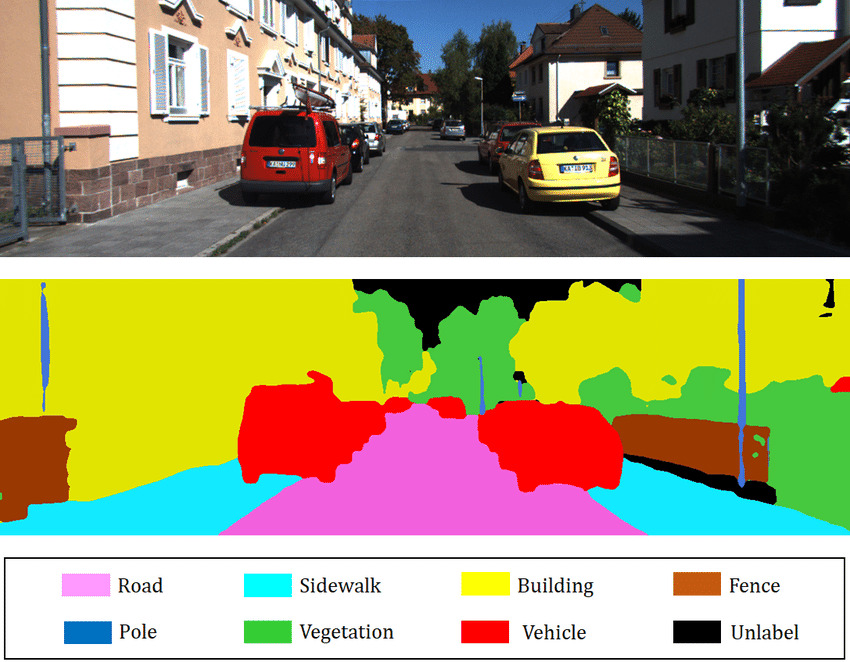
\includegraphics[width=0.9\textwidth]{./assets/semseg.jpg}
    \caption{\label{fig:semseg}Esempio di Semantic Segmentation applicata al riconoscimento di oggetti stradali. Fonte: https://towardsai.net/p/l/machine-learning-7}
\end{figure}

In entrambi i casi, il problema che si tenta di risolvere è detto
{\it semantic segmentation}, di cui un esempio è visibile nella figura \ref{fig:semseg} un caso specifico della {\it image classification}.
Nel secondo caso infatti si classifica un'immmagine interamente come
appartenente a una o l'altra classe, che malpone il problema in essere in
quanto le zone potenzialmente patologiche potrebbero essere anche ridotte
in superficie, quindi facendo prevalere la loro classe rispetto a quella
effettivamente più presente.
Nel secondo caso invece si cercano porzioni dell'immagine che corrispondando a
una specifica classe in modo da poter classificare solo quella porzione.
È dunque un problema che si avvicina molto di più al nostro problema reale
e che ci permette di avere un'idea di come potrebbe essere la nostra soluzione,
nonché essere molto più utile per il personale medico che ha bisogno
di conoscere le zone ritenute come potenzialmente patologiche in modo da
poter valutare effettivamente se lo sia o meno.



% L'$i$-esimo valore del vettore $\vec{y}$, annotato come $y_i$, rappresenta la
% quanto il nostro modello sia convinto che quel dato appartenga alla $i$-esima classe.
% Questo valore non ha un significato fisico reale, semplicemente se $y_0$ è più alto
% di $y_1$, allora per il nostro modello è più probabile che quel dato appartenga alla
% classe $0$. \\
% Si puo' tentare di dare un'interpretazione pribabilistica del significato di $y_i$
% tramite alcuni operatori, con il più utilizzato essere l'operatore {\it softmax},
% definito come:

% $$\displaystyle p_i = \frac{e^{y_i}}{\sum_{j=1}^{N_c} e^{y_j}}$$

% che per via della sua definzione ci assicura che $\displaystyle\sum_i^{N_c} p_i = 1$, ed è
% dunque interpretabile come una distribuzione di probabilità. 
% Una ulteriore possibilità, disponibile nello specifico caso in cui si stia
% lavorando su un problema di classificazione binaria come nel nostro caso,
% è quella di utilizzare un singolo valore in output $y$, con valori di segno
% positivo che indicano un'appartenenza alla classe $C_1$ e valori di segno
% negativo che indicano un'appartenenza alle classe $C_0$.
% La magnitudine di $y$ indica la confidenza del modello nella sua scelta.
% In questo caso, un'operatore che ci permette di dare un significato
% probabilistico ad $y$ è l'operatore {\it sigmoid}, definito come:

% $$\displaystyle p = \frac{1}{1 + e^{-y}}$$

% che indica appunto la probabilità che il dato in input appartenga alla
% classe $C_1$.
% Va da se che per via di questa definzione, $p \in [0, 1]$, e che la probabilità
% che il dato appartenga alla classe $C_0$ è semplicemente $1 - p$.
% Entrambe le opzioni sono attuabili in entrambi i modelli di riferimento,
% e non esiste una regola generica che indichi a priori che uno funzionerà
% meglio dell'altro. \\
% Questa trasformazione in un valore probabilistico non ha un'utilità
% meramente umana, per dare a noi a una misura della confidenza nella
% predizione, ma svolge un suo ruolo in fase di addestramento del modello.
% Di fatto i modelli imparano a riconoscere gli input andando a ridurre il tasso
% di errore, ma non in termini di percentuale di errore o numero assoluto di
% misclassificazioni, ma come cumulativo del totale dell'errore compiuto sulle
% classificazioni.
% La misura di questo errore viene fatta tramite quella che è detta
% funzione di perdita, dalla generica forma $l = L(\vec{y}, \vec{y}^*)$.
% I due modelli di riferimento utilizzano due funzioni di perdita differenti,
% ma una possibile implementazione, molto semplice e spesso dagli scarsi risultati,
% è la differenza dei termini.
% Quindi, se per un campione con $y*=1$ ottenessimo un risultato di $y=0.9$, vale
% a dire modello comunque molto convinto della sua scelta, il nostro errore
% sarebbe quantificabile come $l = |1 - 0.9| = 0.1$.

\subsection{\label{sec:shallow-learning}Tecniche Shallow Learning: Alberi Decisionali}

Il nostro primo modello di riferimento\cite{Toma2022} è basato su
alberi decisionali, modelli molto popolari nel mondo del machine learning
per vari motivi, con il principale essere probabilmente la possibilità
di interpretare il loro funzionamento.
Infatti se con modelli {\it deep learning} non è possibile, se non in
minima misura, aver certezza del processo di apprendimento o interpretare
quello di inferenza, gli alberi decisionali per costruzione sono molto
vicini al pensiero umano, e quindi facilmente interpretabili.
Modelli di questo tipo prendono anche il nome di modelli {\it white box},
mentre modelli non interpretabili prendono il nome di modelli {\it black box}.
Tuttavia, questa affermazione ha una validità relativa, in quanto
nel momento in cui i valori del campione in ingresso, vale a dire le
componenti del nostro vettore $\vec{x}$ salgono in numero e complessità,
questo concetto va via via svanendo.

Il lavoro in questione non ha però semplicemente utilizzato degli decisionali,
ma piuttosto un {\it ensamble} di alberi decisionali, che prende il nome
di {\it random forest}, ovvero un insieme di un grande numero di alberi decisionali.
Questa è una metodologia molto diffusa sopratutto quando, per la difficoltà del
problema o per la scarsità dei dati, non si riesce a costruire un singolo
albero dai risultati soddisfacenti.
Quel che accade è che allora si utilizzano un numero elevati di alberi,
nel concetto generico qui descritti come {\it weak learners}, apprenditori
deboli, e ogni modello esprime la propria valtuazione sul campione.
Viene poi messo in atto un procedimento per ottenere un unico risultato finale,
che nel caso del lavoro descritto è il {\it majority vote}, dove si sceglie
il risultato che la maggioranza dei singoli alberi ha predetto.

\subsection{Algoritmo I}

Al fine di valutare i pro e i contro di questa metodologia, l'algoritmo
è stato reimplementato {\it ex-novo} con una GUI a contorno.
Iniziamo dunque a vederne il funzionamento.\\
L'immagine di partenza viene trasformata in bianco e nero e
suddivisa in blocchi di dimensione prefissata, che prendono il nome di
{\it ROI} ({\it Region of Interest}) o {\it patches}.
La decolorazione è dovuta al fatto che le tecniche di {\it pre-processing},
ovvero le trasformazione applicate all'immagine prima di suddividerla, in {\it ROI},
sono state studiate per immagini in scala di grigi, ma una possibilità potrebbe
essere quella di applicare le stesse tecniche ad ognuno dei canali RGB.\\
Da qui vengono estratti i primi 11 valori statistici che andranno a comporre
i primi 11 valori del nostro vettore $\vec{x}$, che rappresenta la ROI in
ingresso.
A questi vengono poi agginti valori estratti da due matrici che vengono
calcolate dalla ROI stessa, la {\it Gray-Level Co-occurrence Matrix} (GLCM)
e la {\it Gray-Level Run Length Matrix} (GLRLM), che hanno prodotto
risultati soddisfacenti quando applicate ad altri problemi di
{\it pattern recognition}.\cite{GLCM}\\
In entrambi i casi bisogna anzitutto portare l'immagine da scala di grigi
a livelli di grigi.
Un'immagine bianco e nero è composta da un solo canale, con valori che possono
essere rappresentati come numeri interi tra 0 e 255.
Nel caso più generico potremmo dire che un'immagine in bianco e nero
è un'immagine che ha 256 livelli di grigi, ma questo non è ottimale al
funzionamento delle matrici, per cui si digitalizza l'immagine a un numero molto
minore di livelli di grigio, in questo caso 4.
Questo significa che, ai fini del calcolo delle matrici, i valori di grigio
dell'immagine tra 0 e 63, varrà 1 tra 64 e 127, e così via.\\
La GLCM è una matrice quadrata di dimensione $N \times N$, dove $N$ è il
numero di livelli di grigio, che contiene i valori di frequenza con cui
si ripetono coppie di pixel vicini.
È caratterizzata da due parametri, la {\it distanza} $d$ e l'{\it angolo} $\theta$,
ed è possibile utilizzarne molteplici per calcolare più matrici,
ma in questo caso è stata utilizzata una sola matrice, con $d=1$ e $\theta=0$°.
La distanza indica a che distanza cercare la co-occorrenza, nel caso di $d=1$
significa guardare l'elemento adiacente, mentre l'angolo indica la direzione
di adiacenza, in questo caso $0$° quello a destra dell'elemento considerato.

\begin{figure}[h]
    \center
    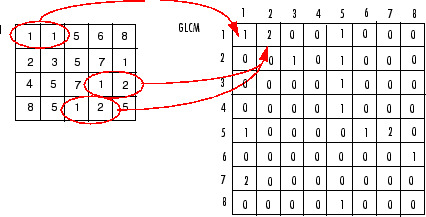
\includegraphics[width=0.9\textwidth]{./assets/glcm.jpg}
    \caption{Illustrazione del Calcolo di una GLCM a 8 livelli di grigio, fonte: https://it.mathworks.com/help/images/create-a-gray-level-co-occurrence-matrix.html}
\end{figure}

Da tale matrice si vanno ad estrarre altri 4 valori statistici.
Segue poi un processo simile per la GLRLM, anch'essa di dimensione
$N \times N$, dove $N$ è nuovamente il numero di livelli di grigio,
ma che è caratterizzata da un solo parametro, l'angolo $\theta$,
che indicia la direzione verso cui viene misurata una {\it run}.
In tale matrice, l'elemento $g_{i,j}$ rappresenta il numero di {\it run}
di lunghezza $j$ percorse nella direzione $\theta$ composte tutte dal medesimo
livello di grigio $i$.
Una rappresentazione visiva del calcolo è riportata nella Figura \ref{fig:glrlm}.

\begin{figure}[h]
    \center
    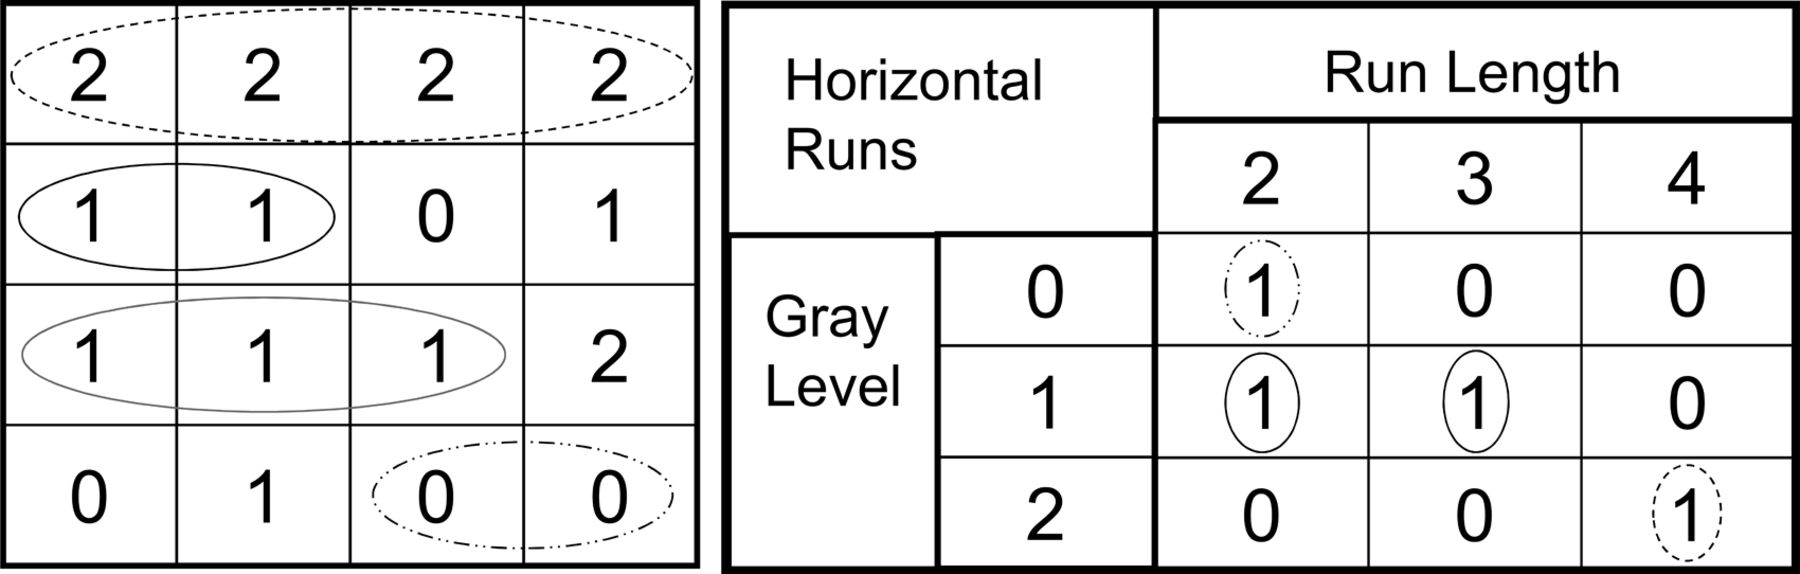
\includegraphics[width=0.9\textwidth]{./assets/glrlm.jpg}
    \caption{\label{fig:glrlm}Calcolo di una GLRLM a 3 livelli di grigio con angolo $\theta$ uguale a 0°, fonte: http://www.ajnr.org/content/36/7/1343/F2}
\end{figure}

Dalla GLRLM si estraggono ulteriori 11 valori statistici.
Infine, l'ultima trasformazione da applicare all'immagine è la traduzione in
dominio di frequenza tramite la {\it Discrete Fourier Transform} (DFT), da cui
si estraggono gli ultimi 3 valori statistici portando il totale a 32.
In tabella \ref{table:features-toma} il dettaglio dei valori statistici impiegati.

\begin{table}
        \center
        \begin{tabular}[h]{||c|c|c|c||}
            \hline 
            \textbf{Primo Ordine} & \textbf{GLCM} & \textbf{GLRLM} & \textbf{DFT} \\
            \hline 
            \hline 
            Media & Contrasto & GLN & Freq. Massima \\
            Mediana & Correlazione & GLNN & Banda \\
            10 Percentile & Energia & HGLRE & Freq. di Kurtosis \\
            90 Percentile & Omogeneità & LGLRE & \\
            Diff. Interquantile & & LRE & \\
            Media Quadratica & & LRHGLE & \\
            Dev. Standard & & LRLGE & \\
            Varianza & & MAD & \\
            Uniformità & & RLN & \\
            {\it Skewness} & & RLNN & \\
            & & RP & \\
            & & SRE & \\
            & & SRHGLE & \\
            & & SRLGLE & \\
            \hline 
        \end{tabular}
        \caption{\label{table:features-toma}Valori statistici estratti dalle ROI.}
    % \end{center}
\end{table}

I valori raccolti da ogni singola ROI vengono raccolti e normalizzati tramite
{\it min-max}. 
Indicando con $max(x,i)$ il valore massimo dell'$i$-esima componente
del vettore $\vec{x}$ presente nel nostro dataset, ed analogamente
per $min(x,i)$, si normalizzano i vettori ricavati da equazione \ref{eq:minmaxnorm}.

\begin{equation}\label{eq:minmaxnorm}
    \vec{x}_{norm} = \frac{\vec{x} - min(x,i)}{max(x,i) - min(x,i)}
\end{equation}

Questo viene fatto perché le varie componenti possono variare molto tra loro
in termini di magnitudine, e potrebbero quindi ingannare gli alberi
a credere che variando di più abbiano un significato maggiore e quindi una
maggiore rilevanza nella classificazione.\\
A differenza di quanto svolto inizialmente in \cite{Toma2022}, la divisione
dei campioni non viene effettuata a posteriori ma a priori:
inizialmente si raccoglievano tutti i campioni e si divdeva in tre parti,
{\it train}, {\it validation} e {\it test}, ma in questo caso si è deciso di optare
per una divisione iniziale delle immagini in questi tre set in modo che
il modello non possa avere indizi extra su una ROI che deve valutare
in fase di test basandosi su una somiglianza di una ROI adiacente o 
parzialmente sovrapposta cui ha avuto accesso in fase di train.

\begin{figure}[h]
    \center
    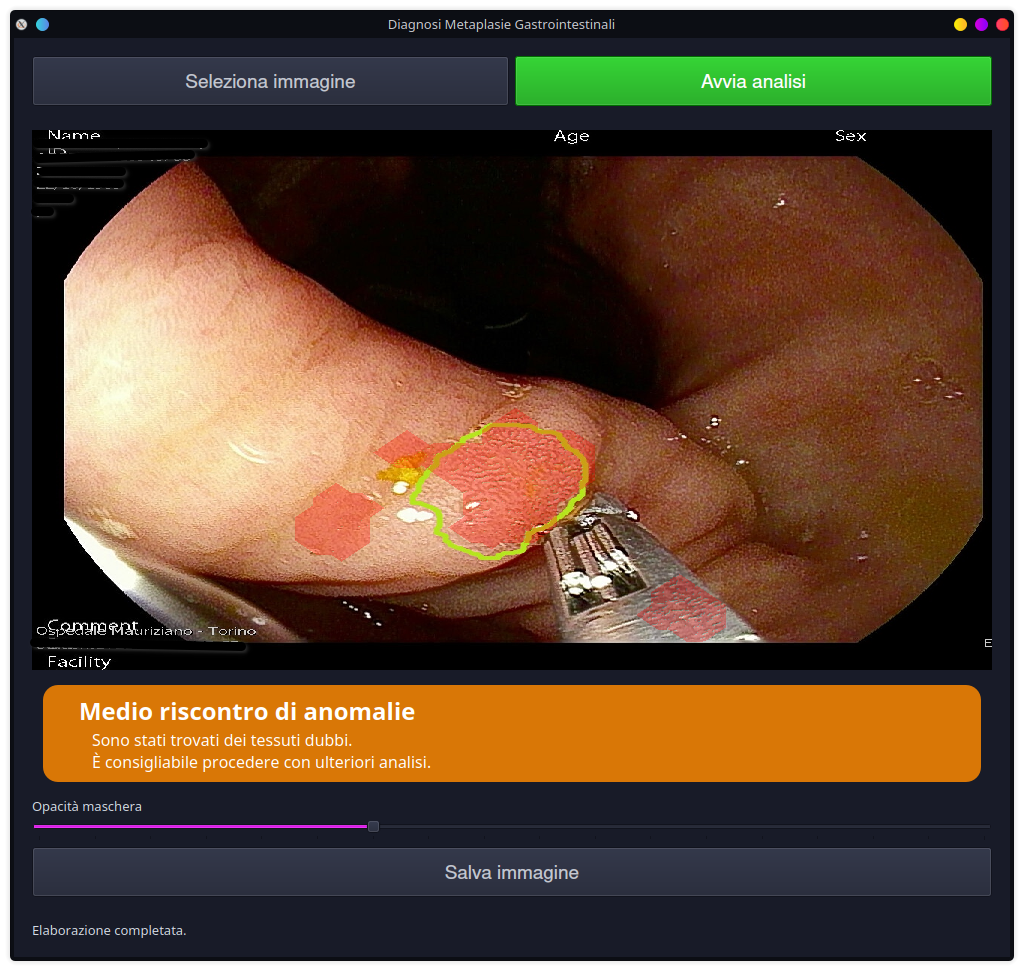
\includegraphics[width=0.9\textwidth]{./assets/gui-one.png}
    \caption{\label{fig:gui-one}Interfaccia grafica per la classificazione delle ROI. La zona cerchiata in verde indica l'area che desidereremmo rilevare, le zone a sovrapposizione rossa indicano le zone rilevate come anomale.}
\end{figure}

A questo punto ogni ROI viene classificata e a partire da essa viene
costruita una maschera globale dell'immagine.
Visto che le ROI vengono estratte con una sovrapposizione spaziale del 40\%,
potremmo avere che alcuni pixel vengano classificati contemporaneeamente
come patologiche che come sane.
Per risolvere questo problema si è classificato il singolo pixel tramite
coefficiente di Dice con soglia impostata a 0.5, che si traduce
praticamente in una classificazione come appartente a una data classe
se la maggioranza delle classificazioni appartengono a quella data classe.
Vengono infine applicati degli operatori morfologi di chiusura, erosione e dilazione
per ottenere una maschera meglio formata.

Presentata questa possibile implementazione abbiamo compreso le grosse
limitazioni che un approccio di questo genere ha.
Per iniziare possiamo notare delle prestazioni da parte del modello non
troppo soddisfacenti.
Una metrica molto utile per comprendere lo scontento è la precisione,
che indica il numero di predizioni corrette sul totale delle predizioni per ogni
classe.
Se quindi per la classe ritenuta sana abbiamo una precisione molto alta, lo stesso
non si puo' dire per quella patologica, che si ferma a circa il 50\%, un valore
troppo basso per un impiego reale.\\
Oltre i problemi di prestazioni, interloquendo con il personale medico
abbiamo idenfiticato ulteriori problemi di natura tecnica.
Il primo, visibile anche il foto, è che l'utilizzo dell'immagine in modalità
bianco e nero faccia perdere moltissime informazioni che potrebbero essere
fondamentali in fase di classificazione.
Ad esempio, come possibile vedere nella figura \ref{fig:gui-one}, un corpo
sicuramente esterno allo stomaco di colore grigio viene in parte
scambiato come tessuto patologico, cosa che difficilmente sarebbe accaduta
utilizzando una versione a colori dell'immagine.\\
Abbiamo poi che l'analisi delle immagini in un secondo momento non risulta
di grande utilità per il personale medico, che ha bisogno di avere un 
riscontro immediato durante l'endoscopia.
Va fatto notare che l'adattamento del modello a funzionare in tempo reale
su un video in input è una strada difficilmente percorribile, in quanto
una prima implementazione dell'algoritmo impiega circa 10 secondi per classificare
la singola immagine.
Quasi l'interità del tempo di elaborazione è speso nel calcolo delle
GLCM e delle GLRLM, dalla mole di calcolo discretamente elevata che aumenta
considerando il grande numero che se ne devono calcolare. \\

In ultimo, grazie al contributo del personale medico, è stato reso evidente
come il considerare le immagini estratte dai 3 filtri che l'I-SCAN utilizza
puo' essere potenzialmente controproducente.
Nello specifico, se nel processo di {\it shuffling}, per pura casualità,
si avesse che vi siano più immagini sane per un dato filtro che per un altro,
potrebbe erroneamente imparare a riconoscere la distribuzione delle
feature estratte da quelle ROI come meno probabilmente patologiche.

\subsection{\label{sec:deep-learning}Tecniche Deep Learning: Reti Neurali Convoluzionali}

Passiamo ora alla seconda possibilità che è stata valutata nello
sviluppare l'applicativo.
Il suo impiego è ispirato dagli ottimi risultati ottenuti in \cite{ilpaper},
che ha dimostrato come un'applicazione di questo tipo possa essere realizzata,
anche se applicandolo al riconoscimento dei polipi, altra patologia
che si sviluppa sempre nello stomaco.
Eventuali differenze di elaborazione verranno spiegate qui, mentre le
differenze nei dati utilizzati verranno spiegate nella sezione \ref{sec:Dataset}.
Vediamo dunque le differenze rispetto al primo algoritmo.
Le reti neurali convoluzionali ricadono, come accennato, nella categoria
{\it black box}.
Questo significa che a differenza del precedente algoritmo non è possibile
comprendere, almeno in modo diretto o semplice, il processo di classificazione,
se non tramite interventi specifici all'architettura interna della rete,
ma solitamente permettono anche di ottenere risultati migliori, soprattutto
nel caso di analisi di immagini in cui hanno sin da principio dimostrato
una grossa dominanza sui modelli di apprendimento superficiale.

La struttura generica di una rete impiegata per la {\it semantic segmentation}
comprende quattro fasi.
La prima è quella di  preprocessing, dove varie trasformazioni vengono applicate
all'immagine in input.
Le trasformazioni più comuni sono la normalazziazione dell'immagine
tramite {\it Z-Normalization}, portando quindi l'immagine in input
ad avere una media di 0 ed una deviazione standard di 1 lungo i tre canali,
oppure altre volte ad aggiungere disturbi nell'immagine, come rotazioni,
desarutazioni e cambi di contrasto casuali al fine di rendere il modello
più robuto ed aumentare artificialmente la quantità di dati di cui si
dispone.
Il dettaglio di quelli applicati è elencato nella sezione \ref{sec:Dataset}.
Trasformazione tassativa è però quella della trasformazione delle dimensioni
dell'immagine a dimensione fissa, perché è necessario che tutte le immagini
siano dello stesso formato.
La seconda fase è quella di {\it feature extraction}, dove il modello
apprende a riconoscere le caratteristiche dell'immagine in input.
Questo avviene tramite l'applicazione di una serie di filtri convoluzionali
e operazioni di {\it pooling} volte a ridurre il numero di dati da usare
in seguito che altramente sarebbe intrattabile.

Il componente che esegue questa estrazione è detta {\it backbone}, ovvero
spina dorsale, e la scelta di quale usale è generalmente libera
ed adattata alle proprie esigenze.
Esistono infatti molteplici backbone, da quelle più semplici che
utilizzano un numero di passaggi limitato, più veloci da elaborare
ma generalmente anche meno performanti, a quelle più complesse che
che invece ottengono risultati migliori al costo di tempo di elaborazione
più elevato.
La scelta di quale usare deve quindi essere un compromesso tra velocità
e accuratezza che va adattato all'applicativo.
Va fatto notare che anche questa fase è soggetta all'apprendimento, ovvero
il modello impara non solo a classificare le aree proposte ma apprende anche
che tipo di aree proporre.

\begin{figure}[ht]
    \centering
    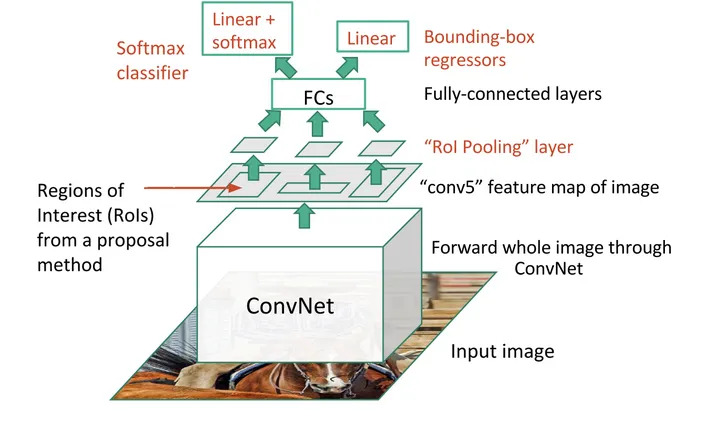
\includegraphics[width=0.9\textwidth]{./assets/cnn.jpg}
    \caption{\label{fig:cnn}Visualizzazione del processo di classificazione di un'immagine. Fonte: https://towardsdatascience.com/region-of-interest-pooling-f7c637f409af}
\end{figure}

L'output di questa fase viene poi sottoposto ad una di {\it region proposal},
dove il modello cerca di individuare nell'immagine delle aree ritenute di
interesse e che vanno quindi analizzate, con delle distinzioni importanti
da fare rispetto all'algoritmo visto in \ref{sec:shallow-learning}.
Se infatti precedentemente si estraevano un numero fisso di ROI e di
dimensione prefissata, in questo caso abbiamo molta più variabilità e
possono dunque essere di numero variabile, generalmente molto più contenuto,
e di dimensione arbitraria.
La ROI proposta viene nuovamente ridmensionata e passata alla testa del
modello, che produce una maschera che classifica il singolo pixel.
Questa è un'ulteriore differenza rispetto a quanto visto prima dove
pixel potenzialmente appartenenti ad un'altra classe venivano classificati
tutti allo stesso modo, mentre in questo caso ogni pixel viene classificato
indipendentemente.
Come accennato, questo era precedentemente accettato poiché le ROI
avevano dimensioni molto contenute e l'obiettivo era classificare l'intera
area di interesse, quindi piccole misclassificazioni non avevano un impatto
significativo.

Notare infne che il modello impara sia a predire la maschera che a
predire la classe da assegnare alla maschera.
Una discussione più dettagliata al nostro caso specifico è fornita
in \ref{sec:results}.

\subsection{Algoritmo II: BiSeNet}

Quelle appena descritte erano le basi generiche del funzionamento
di un modello di deep learning.
Tuttavia le scelte da eseguire in merito sono molteplici, e tra i vari
passaggi possono essere inserite molte variazioni più o meno
significative per ricavare un modello più vicino alle nostre esigenze.
In particolare abbiamo parlato di come la scelta della {\it backbone},
e conseguentemente quindi l'intera procedura di {\it feature extraction},
giochi un ruolo fondamentale nelle prestazioni che si ottengono da un modello.

Se volessimo infatti solo classificare le aree di interesse nel modo
più accurato possibile, magari in un momento distaccato come visto
nel primo approccio, potremmo procedere come appena descritto perché il
procedimento risulterebbe non più lento e la qualità delle predizioni
potrebbe addirittura essere superiori.
Volendo però ottenere tempi inferiori a quelli descritti in
precedenza, non solo inferiori alla decina di secondi ma possibilmente
molto inferiori al secondo, questo non è possibile.

Il modello scelto si chiama {\it BiSeNet}\cite{bisenet}, acronimo di
{\it Bilateral Segmentation Network}, che prende il nome per via
della sua architettura interna che si dirama in due parti.
Come discusso, la scelta della {\it backbone} di un modello, e più
precisamente delle caratteristiche che puo' offrire,
porta con sé grosse implicazioni sul tipo di prestazioni che si
possono ottenere.
Questo dipende anche dal fatto che le {\it backbone} stesse possono
essere costruitre per ottenere un dato risultato piuttosto che un
altro.
In alcuni casi architetture più pesanti, facendo uso di molti
livelli convoluzionali detti a piramide riescono a comprimere
con efficacia l'informazione presente nell'immagine,
tentando di compensare la lentezza andando ad operare su un
input di dimensioni ridotte, che comporta di per sè una perdita
di informazione.
Altre invece fanno uso di {\it pooling} aggressivi, che riducono
velocemente la dimensione dell'input e codificano meglio
dettagli di alto livello e sono quindi veloci ad elaborarlo.

\begin{figure}
    \center
    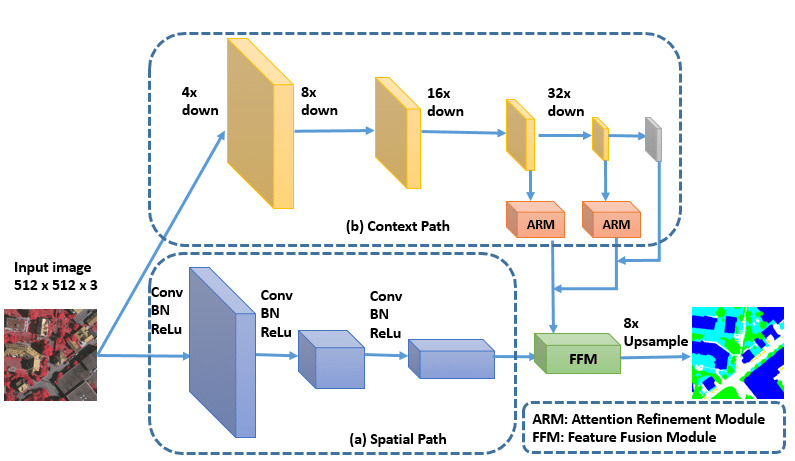
\includegraphics[width=0.9\textwidth]{./assets/bisenet.jpg}
    \caption{\label{fig:bisenet}Visualizzazione ad alto livello dell'architettura di BiSeNet. Fonte: researchgate.net}
\end{figure}

È quindi evidente che oltre una scelta in termini di rapidità
vi è anche da considerare che tipo di informazione si stia cercando
di estrarre dall'immagine, ma pare subito evidente che per una
classificazione realmente soddisfacente puo' risultare necessario
utilizzare entrambi.
BiSeNet quindi implica entrambe le strategie, con quelle che sono
dette {\it Spatial Path} e {\it Context Path}.
Nel primo caso si utilizzano un numero elevato di livelli
convoluzionali per codificare quanta più informazione spaziale possibile,
nel secondo caso si comprime l'informazione di alto livellot tramite
meccanismi di pooling e filtri convoluzionali di dimensione ridotta.
L'output della {\it Context Path} viene poi sottoposto a dei
meccanismi di attenzione per selezionare quali dettagli di alto
livello tra quelli catturati possa essere il più rilevante, e
e successivamente tramite quel che è detto {\it Feature Fusion
Module} viene unito all'output della {\it Spatial Path}, che
in questa fase svolge il ruolo della testa.
L'output viene dunque riscalato in modo da avere dimensioni
uguali a quelle proposte in input.

\section{\label{sec:Dataset}Dataset}

Allenando un modello di intelligenza artificiale è necessario
rifelttere su quali dati si stiano utilizzando.
Il già grande e tutt'ora crescente interesse per la disciplina
nel mondo della ricerca ha infatti portato alla raccolta
e pubblicazione di grandi dataset per sperimentare
nuove tecniche e avere dei confronti di prestazioni
normalizzati tra i differenti modelli.
Tuttavia, puntanto a costruitre un applicativo che possa essere
considerato come qualcosa di concretamente reale, non è
spesso possibile utilizzare questi dataset, perché
spesso non sono disponibili dati specifici per l'applicativo
in considerazione o quelli disponibili non sono rappresentativi
del nostro caso.

Ci sono anche casi in cui si dispone invece dei dati, ma
essi sono semplicemente troppo pochi.
sebbene tecniche di {\it data augmentation}, ossia tecniche
che puntano ad aumentare in maniera artificiale la quantità
di dati di cui si discone, portando in realtà anche un
aumento della qualità del modello prodotto, siano la norma
nello sviluppo di un modello, se comunque i dati a disposizione
sono in partenza di quantità molto scarsa non è possibile
sperare di ottenere un modello robusto e affidabile.
Per questo motivo in questo progetto sono stati usati due
dataset, uno pubblico e noto all'interno della comunità
della ricerca e l'altro composto da immagini raccolte e
annotate dall'Ospedale Mauriziano di Torino.

\subsection{\label{sec:dataset-mauriziano}Il Dataset Mauriziano}

Il dataset si compone di 113 immagini di esami endoscopici
raccolte dall'ospedale Medico durante le loro attività,
di cui 51 con aree patologiche e 62 senza.
Si presentano come acquisizioni del macchinario I-Scan,
e quindi sono immagini ad altissima risoluzione (1920$\times$1080 pixel).
Essendo però acquisizioni del macchinario, presentano anche
una grandissima quantità di informazioni superflue o non utilizzabili,
come grosse porzioni di immagini nere che in realtà fanno parte
dell'interfaccia oppure una seconda visuale ausiliaria che non
puo' essere impiegata al fine dell'addestramento del modello.
Questo porta la porzione di immagine realmente utilizzabile
a circa 1250$\times$1020, una risoluzione comunque molto
elevata.

Tuttavia, per una questione numerica, questo non puo' essere
l'ultimo dataset impiegato.
Delle 51 immagini patologiche annotate infatti di solo 
18 si dispone anche dell'immagine originale non annotata.
Va fatto notare che le annotazioni sono state eseguite in maniera
{\it hard coded} sull'immagine, e non è quindi separabile dall'immagine
originale.
Questo non è un problema per l'addestramento del modello descritto
nella sezione \ref{sec:shallow-learning} in quanto la conversione
dell'immagine in scala di grigi e l'utilizzo di porzioni di immagini
molto ridotte non permette al modello di discriminare le ROI
in base alla presenza o meno di questa annotazione.
Nel caso del modello descritto nella sezione \ref{sec:deep-learning}
invece è molto possibile che il modello impari a proporre le ROI,
se non direttamente a classificarle in base alla presenza
dell'annotazione, in quanto sarebbe in grado di riconoscere
la differenza di colore e discriminare le ROI in base a questo.

\begin{figure}[h]
    \center
    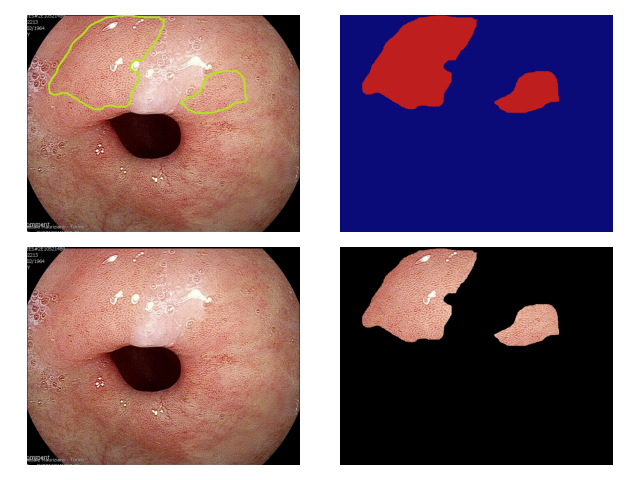
\includegraphics[width=0.9\textwidth,trim=5.0cm 5cm 6cm 6.0cm,clip]{./assets/cutout.png}
    \caption{\label{fig:cutout}Processo di estrazione di una ROI. Da sinistra a destra:
    Immagine originale, maschera calcolata, visualizzazione della sola area patologica
    }
\end{figure}

La creazione della maschera è possibile tramite delle semplici
considerazioni sulla natura delle annotazioni, in quanto sono
state fatte con l'utilizzo di un verde tipicamente ad alto
contrasto con il resto delle immagini.
Per via di questa caratteristica è facile ottenere una prima
{\it bitmap} del marchio apposto sulla foto.
Successivamente si applicano in sequenza i seguenti operatori
binari:

\begin{itemize}
    \item {\it Dilatazione}: chiusura di eventuali aree non congiunte
    \item {\it Chiusura}: riempire il centro dell'annotazione
    \item {\it Erosione} $\times$ 2: annullamento della precedente dilatazione
    e restringimento della maschera all'interno dell'annotazione
\end{itemize}

Nel caso dell'algoritmo in \ref{sec:shallow-learning} dalle immagini
elaborate vengono estratte ROI di dimensione 50 $\times$ 50 pixel,
con una sovrapposizione del 40\%, ovvero 20 pixel.
Per aumentare la quantità di ROI patologiche di cui si è a disposizione
esse vengono inoltre salvate anche rotate di 90°.
Questo permette di estrarre in totale circa 210'000 campioni su cui allenare
il modello.
È bene notare che nonostante questo tentativo di aumentare le ROI
patologiche viene applicato alle immaigni non-patologiche un processo
di {\it oversampling}, ovvero in fase di estrazione delle {\it features}
alcune ROI sane vengono estratte più di una volta, in quanto questo
ha sperimentalmente prodotto un modello più oggettivo nelle sue
valutazioni.

\begin{table}
    \center
    \begin{tabular}[h]{||c||c|c|c||}
        \hline
        & Train & Test & Totale \\
        \hline
        Immagini Sane & 40 & 7 & 47 \\
        \hline
        Imagini Patologiche & 42 & 6 & 48 \\
        \hline
        ROI Sane & 84'847 & 6'657 & 91'504 \\
        \hline
        ROI Patologiche & 54'278 & 1'620 & 55'898\\
        \hline
        \hline
        \multirow{2}{*}{Totale} & 82 & 13 & 95 \\ \cline{2-4}
        & 149'548 & 64'442 & 213'990 \\
        \hline
    \end{tabular}
    \caption{\label{tab:mauriziano}Composizione del dataset Mauriziano}
\end{table}

Nel caso dell'algoritmo in \ref{sec:deep-learning} invece, le immagini
vengono solo ridimensionate a una dimensione di di 570 $\times$ 570 pixel,
ruotate orizzontalme in maniera casuale con una probabilità del 50\%.
Questo è fatto perché vengono utilizzate assieme alle immagini
dell'altro dataset e devono quindi avere la stessa dimensione.
Data la risoluzione ridotta delle immagini, è più conveniente
ridimensionare queste che invece sono di risoluzione più alta.

\begin{figure}
    \center
    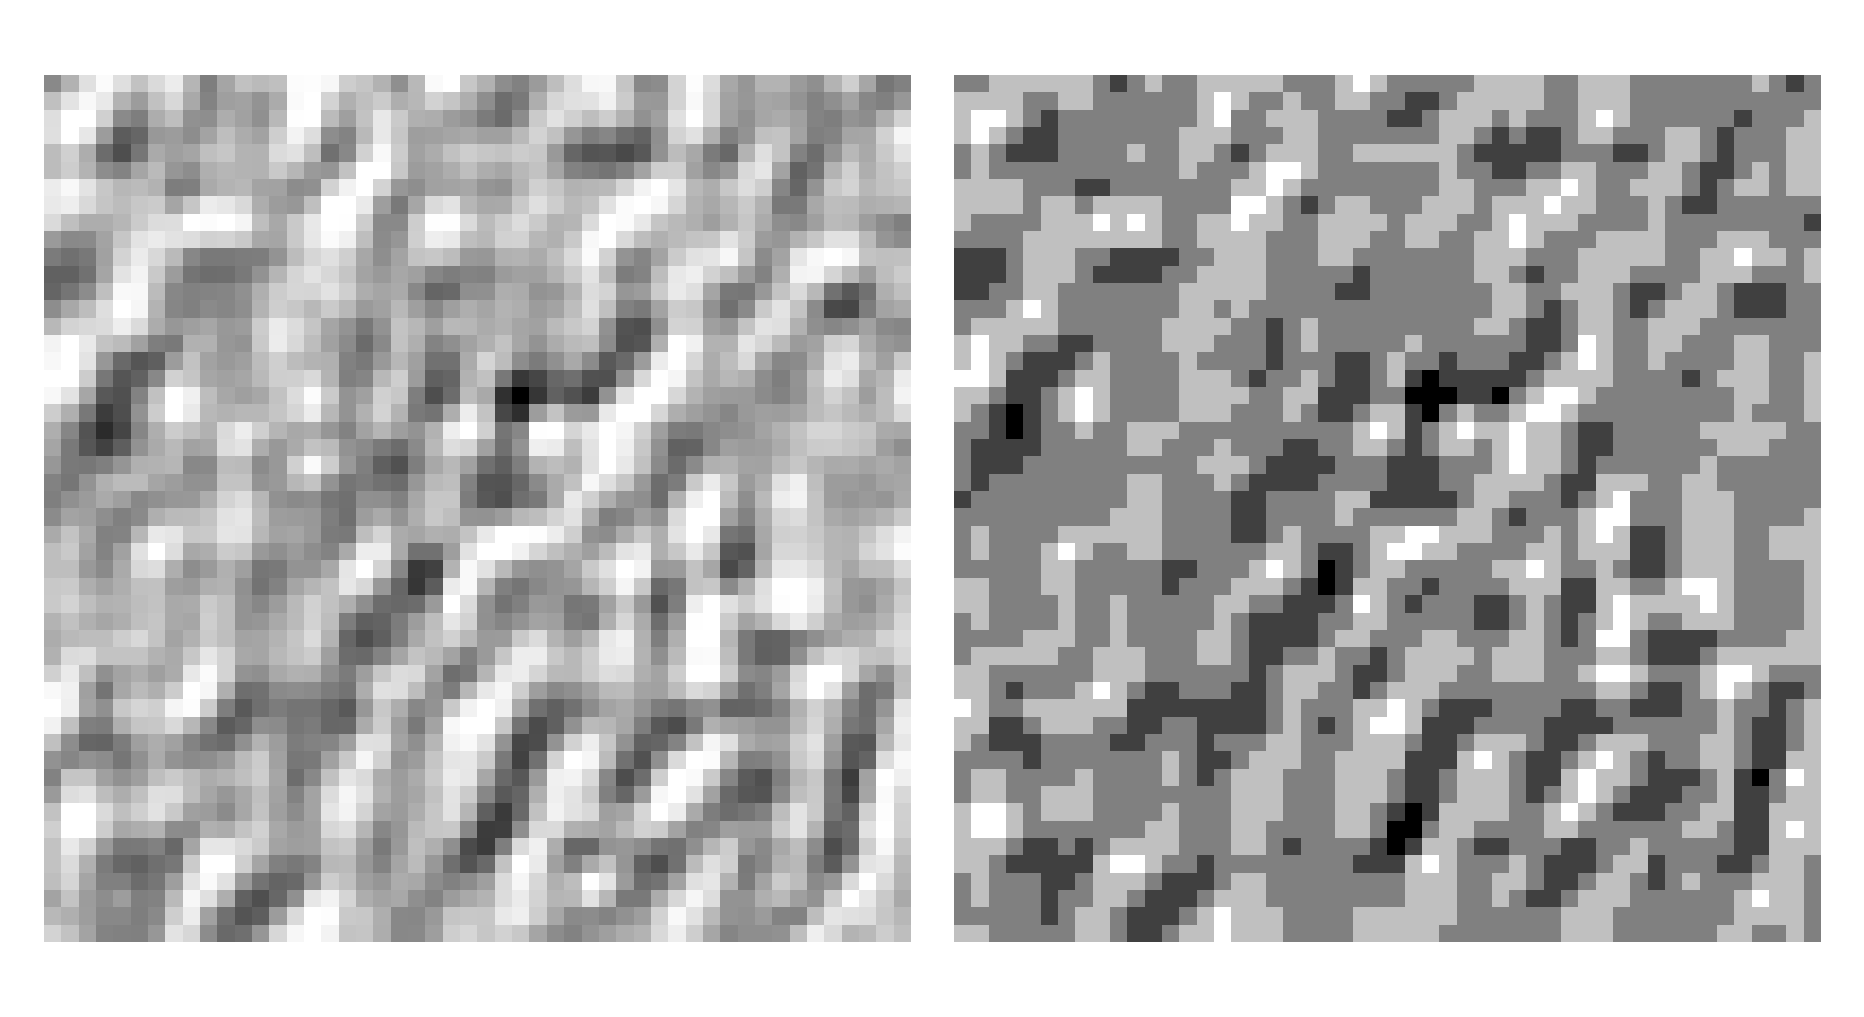
\includegraphics[width=0.9\textwidth]{./assets/roi-shallow.png}
    \caption{\label{fig:roi-shallow} Esempio di ROI estratta per algoritmo di shallow learning (sinistra) e
    di versione digitalizzata su 5 livelli di grigio per il calcolo di GLCM e GLRLM (destra).}
\end{figure}

\subsection{Il Dataset HyperKvasir}

Il dataset HyperKvaris\cite{HyperKvasirDataset} nasce per sopperire
alla mancanza di dati medici per lo studio e l'addestramento
di modelli di intelligenza artificiale.
La raccolta di dati è, in ogni ambito, un lavoro costoso non 
soltatno in termini monetari ma spesso e volentieri anche
per fattori di tempo e di risorse umane.
Dataset comunemente usati nella ricerca di modelli di intelligenza
artificiale, come {\it Common Object and Context}\cite{cocodataset}
(COCO) ed {\it ImageNet} \cite{imagenet} contengono
immagini di oggetti comuni presi dalla quotidianità,
quindi classificabili da qualunque persona: ciò non toglie
che il processo di annotazione, che puo' prendere
varie forme come la classificazione, la segmentazione e la
circoscrizione, sia un processo lungo e ripetitivo.

Nel caso specifico della medicina, le cose si complicano
molto di più.
Sin dal principio, è molto diffile ottenere i dati grezzi,
quindi non annotati, spesso anche per tutelare la privacy
del paziente stesso, o comunque è difficile ottenerne in
quantità sufficienti, ed anche quando questo accade
è necessario l'impiego di personale medico altamente
specializzato, nel nostro caso nel settore della
gastroenterologia, per annotare e segmentare le immagini.
Specificiatamente per l'ambito medico, è anche preferibile
avere più di un riscontro.

HyperKvasir è dunque la più grande raccolta di immagini
e video di esami di endoscopia digestiva, rilasciato proprio
allo scopo di facilitare la ricerca in questo ambito.
Va fatto tuttavia notare che quanto detto in precedenza resta
purtroppo vero:
non lasciandoci trarre in inganno dalla dimensione del dataset,
che ammonta a ben 110'00' immagini e 374 video, bisogna
constatare che si tratti comunque di un dataset molto
eterogeno nella sua composizione.
Delle 110'000 immagini, infatti, 99'000 sono che sono
talmente prive di annotazioni, vale a dire nè classificate
nè segmentate in alcun modo, e delle restanti 11'000
solo 1'000 sono immagini di cui sono disponibili
le annotazioni di segmentazione.
Per ultimo, trattandosi di un dataset per lo studio
di analisi endoscopiche, le immagini riportanti metaplasie
sono presenti solo come immagini classificate ma non come
segmentate, fattore che renderebbe impraticabile
l'utilizzo del nostro modello.

\begin{table}
    \center
    \begin{tabular}{||c|c|c|c||}
        \hline
        Tipologia & Quantità & Descrizione & Dimensione (MB) \\
        \hline
        \hline
        Classificate & 10'662 & 23 classi & 3'960 \\
        \hline
        Segmentate & 1'000 & Solo polipi & 57 \\
        \hline
        Non annotate & 99'417 & Non annotate & 29'940 \\
        \hline
        Video & 374 & 30 classi di appartenenza & 32'539 \\
        \hline
        \hline
        Totale & 111'453 & --- & 66'496 \\
        \hline
    \end{tabular}
    \caption{\label{tab:hyperkvasir}Composizione del dataset HyperKvasir}
\end{table}

È ovviamente improprio l'utilizzo di un dataset riportante
classi diverse da quelle che si possono riscontrare nel 
contesto di applicazione per l'addestramento del modello,
tuttavia avendo a che fare con un numero di campioni
relativo ad esso molto limitato si è scelto di utilizzarlo
in congiunzione con il dataset descritto in \ref{sec:dataset-mauriziano}.
Questo è possibile tramite l'impiego del {\it transfer learning},
che consiste nell'usare come base di partenza per l'addestramento
di un nuovo modello uno già allenato su un dataset con
caratteristiche simili al nuovo.
Questa tecnica è generalmente utilizzata per velocizzare
il processo di apprendimento, insieme anche al raggiungimento
di risultati migliori, ma è anche molto utile quando si 
dispone di pochi dati, come nel nostro caso.
È bene notare dunque che l'impiego di {\it transfer learning}
per lo sviluppo di modelli di intelligenza artificiale non è
dunque un ultima risorsa ma bensì la norma, vista la
pervasività che ha dimostrato nei vari ambiti di applicazione.

In ultimo, il dataset HyperKvasir è anche molto eterogeno
nella forma in cui si presentano le immagini.
A differenza del dataset in \ref{sec:dataset-mauriziano} infatti,
dove le acquisizioni sono state effettuate tutte con la medesima
macchina, sono di uguale ed altissima risoluzione, nel caso
di HyperKvasir infatti abbiamo con immagini provenienti da diverse
fonti e di qualità generalmente inferiore.

%% \begin{table}
    %% \center
    %% \begin{tabular}{||c|c|c|c|c||}
        %% \hline
        %% & W < 400 & 400 < W < 600 & 600 < W < 800 & W > 800 \\ 
        %% \hline
        %% H < 400 &  &  &  & \\ 
        %% \hline
        %% 400 < H < 800 &  &  &  & \\ 
        %% \hline
        %% 600 < H < 800  &  &  &  & \\ 
        %% \hline
        %% H > 800 & &  &  & \\ 
        %% \hline
    %% \end{tabular}
%% \end{table}

\section{Processi}
\subsection{La Libreria MMSegmentation}
\subsection{Allenamento del Modello}
\subsection{Valutazione del Modello}